%-----------------------------------------------------------------------------
%
%          PHYSICS  M.S.     THESIS
%          JUSTIN A. VASEL
%
%          This began as the template offered by the University of Minnesota, 
%          but I've made a few changes here and there...  
%
%          -->  halo2.tex
%
%-----------------------------------------------------------------------------


\chapter{The Road to Full Operation}
	\label{halo2_chapter}

	\begin{quoting}
		\noindent \large ``For tomorrow belongs to the people who prepare for it today." \normalsize

		--- African Proverb
	\end{quoting}

	\chapterIntro{I}{arrived at SNOLAB to begin work on HALO in July of 2012.} Construction of the detector hardware had finished not long before that and the detector had been running and collecting data since May of 2012. However, HALO was far from being ready to do its job. Many vital components were missing: SNEWS alert triggers were not developed, hardware redundancy was not in place, there was no way to remotely monitor the hardware, and the detector had not yet been calibrated. 

	My job at HALO was not singularly data analysis nor theoretical research nor computer simulation. My contribution to the experiment was more vague and arguably more involved: to help the collaboration move through this laundry list of tasks in a timely manner so that HALO will be ready to serve its purpose before the next galactic supernova occurs. In this chapter, I will discuss my involvement in preparing the Helium and Lead Observatory for full operation.

	\section{Identifying Faulty{}\he Counters}
		As mentioned in \CHP \ref{halo_chapter}, the{}\he proportional counters were donated to HALO by the decommissioned SNO experiment. Only 128 counters are required for HALO, which left us with a couple dozen extra to be kept on reserve in case a counter in the detector for whatever reason needs to be replaced. The neutron spectrum for each counter currently in the detector had been carefully examined to ensure the active counters were behaving as expected, but the extra counters had not yet been so thoroughly vetted. It was known that some of the counters were filled with $^4$He gas, which cannot be used in the detection of neutrons. The SNO experiment used these as a control group and they got mixed in with the{}\he counters when they were delivered to HALO. 

		To identify the $^4$He counters in the group and to ensure that the{}\he counters were behaving normally, we tested each of them by collecting and examining their neutron spectrum. To avoid disrupting any of the 128 active counters in the detector during testing, we ran wiring from the storage rack to the rest of the hardware. This allowed us to test four counters at a time while the rest of the detector ran normally.

		Most counters were allowed to accumulate data for several days before inspection. A healthy{}\he counter displayed a statistically significant neutron peak located near an ADC value of 1,000\footnote{At this point, the arbitrary ADC value scale for energy had not been mapped to keV. Such a mapping depends on the peculiarities of the{}\he counter, the gains within it, and thresholds applied to it. An algorithm to perform this conversion for each counter is currently in development.} and a tall and sharp gamma peak at very low energies (\FIG \ref{fig:halo_neutron_spectra}, left). An unhealthy{}\he counter may have a broadened neutron peak or other strange artifacts in the spectrum (\FIG \ref{fig:halo_neutron_spectra}, center). A $^4$He counter would simply not have the neutron peak (\FIG \ref{fig:halo_neutron_spectra}, right).
		\begin{figure}[H]
			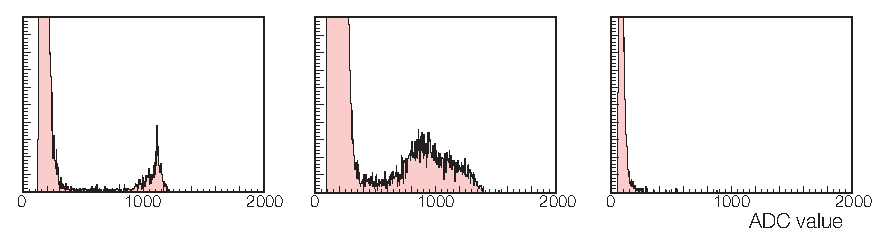
\includegraphics[width=\textwidth]{halo_neutron_spectra}
			\caption[Neutron Counter Response]{\bf Neutron counter response. \rm A healthy{}\he counter \emph{(left)} exhibits a sharp neutron peak and a gamma peak. An unhealthy{}\he counter \emph{(center)} also has a gamma peak, but may show a broadened neutron peak or other obscure features. A $^4$He counter \emph{(right)} features a gamma peak, but no neutron peak.}
		\label{fig:halo_neutron_spectra}
		\end{figure}

		After characterization, we identified both healthy and unhealthy{}\he counters and the $^4$He counters. \confirm{A \he counter with a gas leak will experience a decrease in gain} and manifest itself as a distorted neutron spectrum. We suspected that any unhealthy spectra we found would be due to such a leak, but after finding several of these, we began to wonder if there was another explanation. It was a symptom worthy of further investigation, in case it could affect healthy{}\he detectors down the road.
	\section{DAQ Software Development}
		\filler
	\section{Remote Monitoring}
		\filler
	\section{Current Status and Future Work}
		\filler


%-----------------------------------------------------------------------------
%-----------------------------------------------------------------------------